\chapter{Janus protocol}
Na sběrnici RS-485 se nabízela možnost použít protokol Modbus \cite{modbus}, což je průmyslový standard.
Byla to původně i moje volba, ale v~době, kdy jsem s~prací začínal, nebyl ještě Modbus na ESP32 oficiálně podporován.
Rozhodl jsem se proto vytvořit vlastní protokol, pracovně pojmenovaný Janus protocol.
Nyní, i přestože je Modbus na ESP32 již podporován, jsem se rozhodl u~Janus protocol zůstat, protože je oproti Modbus jednoduší.
Zároveň se díky tomu nebudu muset starat o~udržení kompatibility s~Modbusem.
Další z~důvodů byla neexistence některých parametrů v~hlavičce Modbusové zprávy, jako například adresa odesílatele. 

Janus protocol je snaha o~vytvoření uživatelsky co nejpřívětivějšího a zároveň robustního protokolu.
Tento protokol je postavený z~velké části na Avakar protokolu.
Přidává k~němu adresaci zpráv a CRC16.


\section{Základní specifikace}
\begin{itemize}
    \item Multi-slave
    \item Podpora zpráv různých délek -- při zachování minimální délky/hlavičky
    \item Až 254 zařízení (limitováno RS-485 na 32/128 zařízení -- bez použití rozbočovačů)
    \item Jednoduché přidání dalšího senzoru do již zavedeného systému
\end{itemize}

Janus protocol používá 7-bytovou hlavičku následovanou datovými byty, těch může být teoreticky až 255.
Viz obrázek \ref{fig: Diagram protokolu}.

Hlavička sestává ze startovacího bytu, ten je statický a má hodnotu vždy 0x80.
Následuje adresa adresáta, zařízení, pro které je správa určena.
Pokud je tato adresa rovna 0xFF, jedná se o broadcastovou zprávu. To znamená, že ji přijmou všechna zařízení, odpovědět na ni však může pouze jedno.
Na třetí pozici je adresa odesílatele zprávy.
Na pozici čtvrté je číslo příkazu, ten říká zařízení jak má se správou naložit.
Následuje byte určující počet datových bytů.
Na šesté a sedmé pozici se nachází 16-bitové CRC.

Datové byty přenáší parametry pro příkaz určený číslem příkazu v hlavičce.
To mohou být jak nastavovací hodnoty pro senzory, tak hodnoty vracené ze senzorů do řídící jednotky.

\begin{figure}[h]
    \begin{small}
        \begin{center}
            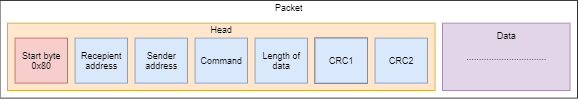
\includegraphics[width=400px]{img/Protocol_diagram.png}
        \end{center}
        \caption{Diagram protokolu}
        \label{fig: Diagram protokolu}
    \end{small}
\end{figure}


Kompletní implementace protokolu pro ESP32 je dostupná na serveru Github \cite{protocol}. 


